\documentclass[epsfig,10pt,fullpage]{article}

\newcommand{\LabNum}{2}
\newcommand{\CommonDocsPath}{../../common/docs}
\addtolength{\textwidth}{1.5in}
\addtolength{\oddsidemargin}{-0.75in}
\addtolength{\topmargin}{-0.75in}
\addtolength{\textheight}{1.5in}
\addtolength{\evensidemargin}{0.75in}
\setlength\parindent{0pt}
\raggedbottom

\usepackage{ae,aecompl}
\usepackage{epsfig,float,times}
\usepackage[hypcap]{caption}
\usepackage[pdftex, colorlinks]{hyperref}
\usepackage{graphicx}
\usepackage[usenames, dvipsnames]{color}
\usepackage{rotating}
\usepackage{tikz}
\usetikzlibrary{automata,positioning}
\usepackage{placeins}

\widowpenalty 10000
\clubpenalty 10000

\newcommand{\red}[1]{{\color{red}\sf{#1}}}
\newcommand{\green}[1]{{\color{green}\sf{#1}}}
\newcommand{\blue}[1]{{\color{blue}\sf{#1}}}
\definecolor{PineGreen}{rgb}{0.0, 0.47, 0.44}
\definecolor{ForestGreen}{rgb}{0.13, 0.55, 0.13}
\definecolor{Brown}{rgb}{0.59, 0.29, 0.0}

\newcommand{\UPDatePublished}{Oct 2021}
\newcommand{\versnum}{21.1} %version number quartus/AMP
\newcommand{\quartusname}{Quartus\textsuperscript{\textregistered} Prime}	
\newcommand{\UPTextBar}{For \quartusname{} \versnum{}}
\newcommand{\thisyear}{2021 } %for copyright
\newcommand{\company}{FPGAcademy.org}
\newcommand{\longteamname}{FPGAcademy.org}
\newcommand{\teamname}{FPGAcademy}
\newcommand{\website}{FPGAcademy.org}

\newcommand{\productAcronym}{AMP}
\newcommand{\productNameShort}{Monitor Program}

\newcommand{\productNameMedTM}{A Monitor Program}
\newcommand{\productNameMed}{A Monitor Program}

%\newcommand{\headerLogoFilePath}[1]{#1/FPGAcademy.png}

% listings is a package that supports encapsulating source code in LaTeX conveniently
\usepackage{listings}

\def\expandparam\lstinputlisting[#1]#2{\edef\tmp{\noexpand\lstinputlisting[#1]{#2}}\tmp}

%%%%%%%%%%%%%%%%%%%% Source Code Formatting %%%%%%%%%%%%%%%%%%%%
\definecolor{globalCommentColour}{rgb}{0.588,0.588,0.588}

%%%%%%%%%%%%%%%%%%%%%%%%%%%%%%%%%%%%%%%%%%%%%%%%%%%%
% Defining language style
% NiosII ASM
\lstdefinelanguage[NiosII]{Assembler} {
  morekeywords={add, addi, and, andhi, andi, beq, bge, bgeu, bgt, bgtu, ble,  bleu, blt, bltu, bne, br, break,
  bret, call, callr, cmpeq, cmpeqi, cmpge, cmpgei, cmpgeu, cmpgeui, cmpgt, cmpgti, cmpgtu, cmpgtui, cmple,
  cmplei, cmpleu, cmpleui, cmplt, cmplti, cmpltu, cmpltui, cmpne, cmpnei, custom, div, divu, eret, flushd,
  flushda, flushi, flushp, initd, initda, initi, jmp, jmpi, ldb, ldbio, ldbu, ldbuio, ldh, ldhio, ldhu, ldhuio,
  ldw, ldwio, mov, movhi, movi, movia, movui, mul, muli, mulxss, mulxsu, mulxuu, nextpc, nop, nor, or, orhi, ori,
  rdctl, rdprs, ret, rol, roli, ror, sll, slli, sra, srai, srl, srli, stb, stbio, sth, sthio, stw, stwio,
  sub, subi, sync, trap, wrctl, wrtcl, wrprs, xor, xori, xorhi, xori},
  morekeywords=[2]{.abort, .ABORT, .align, .app-file, .ascii, .asciz, .balign, .byte, .comm, .data, .def,
  .desc, .dim, .double, .eject, .else, .end, .endef, .endif, .equ, .equiv, .err, .extern, .file, .fill, .float,
  .global, .globl, .hword, .ident, .if, .include, .int, .irp, .irpc, .lcomm, .lflags, .line, .linkonce, .ln,
  .list, .long, .macro, .mri, .nolist, .octa, .org, .p2align, .psize, .quad, .rept, .sbttl, .scl, .section,
  .set, .short, .single, .size, .sleb128, .skip, .space, .stadb, .stabn, .stabs, .string, .symver, .tag,
  .text, .title, .type, .val, .uleb128, .word},
  morekeywords=[3]{et, bt, gp, sp, fp, ea, sstatus, ra, pc, status, estatus, bstatus, ienable, ipending, cpuid,
  exception, pteaddr, tlbacc, tlbmisc, eccinj, badaddr, config, mpubase, mpuacc},
  sensitive=t,
  alsoletter=.,
  morestring=[b]",
  morecomment=[s]{/*}{*/},
  morecomment=[l]\#,
}[keywords,comments,strings]
   
%% NOTE: morekeywords=[2] are GNU directives.
   
\definecolor{niosInstructionColour}{rgb}{0.000,0.608,0.000}
\definecolor{niosDirectiveColour}{rgb}{0.000,0.000,0.902}
\definecolor{niosSpecialRegColour}{rgb}{0.000,0.000,0.000}
\definecolor{niosStringColour}{rgb}{0.808,0.482,0.000}
   
%% NOTE: To make bold use: =\bfseries\color{<colour>}
\lstdefinestyle{defaultNiosStyle} {
  language=[NiosII]{Assembler},
  stringstyle=\color{niosStringColour},
  keywordstyle=\color{niosInstructionColour},
  keywordstyle=[2]\color{niosDirectiveColour},
  keywordstyle=[3]\itshape\color{niosSpecialRegColour}
}
%%%%%%%%%%%%%%%%%%%%%%%%%%%%%%%%%%%%%%%%%%%%%%%%%%%%

%%%%%%%%%%%%%%%%%%%%%%%%%%%%%%%%%%%%%%%%%%%%%%%%%%%%
% Defining language style
% ArmA9 ASM
\lstdefinelanguage[ArmA9]{Assembler} {
  morekeywords={ADC, ADD, ADDS, AND, ANDS, B, BAL, BEQ, BGE, BGT, BL, BLT, BIC, BKPT, BLX, BNE, BX, CDP, CLZ, CMN, CMP, EOR,
  EORS, LDC, LDM, LDR, LDRB, LDRBT, LDRH, LDRSB, LDRSH, LDRT, LSL, MCR, MLA, MOV, MOVW, MOVT, MRC, MRS, MSR, MUL, MVN, ORR, PLD,
  ROR, RSB, RSC, SBC, SMLAL, SMULL, STC, STM, STR, STRB, STRBT, STRH, STRT, SUB, SUBS, SWI, SWP, SWPB, TEQ, UMLAL,
  PUSH, POP, MOVS, RORS, LSR},
  morekeywords=[2]{.abort, .ABORT, .align, .app-file, .ascii, .asciz, .balign, .byte, .comm, .data, .def,
  .desc, .dim, .double, .eject, .else, .end, .endef, .endif, .equ, .equiv, .err, .extern, .file, .fill, .float,
  .global, .globl, .hword, .ident, .if, .include, .int, .irp, .irpc, .lcomm, .lflags, .line, .linkonce, .ln,
  .list, .long, .macro, .mri, .nolist, .octa, .org, .p2align, .psize, .quad, .rept, .sbttl, .scl, .section,
  .set, .short, .single, .size, .sleb128, .skip, .space, .stadb, .stabn, .stabs, .string, .symver, .tag,
  .text, .title, .type, .val, .vectors, .uleb128, .word},
  morekeywords=[3]{SP, PC, MIDR, CTR, TCMTR, TLBTR, MPIDR, ID_PFR0, ID_PFR1, ID_DFR0, ID_MMFR0, ID_MMFR1, ID_MMFR2,
  ID_MMFR3, ID_ISAR0, ID_ISAR1, ID_ISAR2, ID_ISAR3, ID_ISAR4, CCSIDR, CLIDR, AIDR, CSSELR, TTBR0, TTRB1, TTBR2, DACR,
  DFSR, IFSR, ADFSR, AIFSR, DFAAR, IFAR, ICIALLUIS, BPIALLIS, PAR, ICIALLU, ICIMVAU, BPIALL, DCIMVAC, DCISW, V2PCWPR,
  DCCVAC, DCCSW, DDIMVAC, DCISW, TLBALLIS, TLBIMVAIS, TLBIASIDIS, TLBIMVAAIS, TLBIALL, TLBIMVA, TLBIASID, TLBIMVAA,
  PMCR, PMCNTENSET, PMCNTENCLR, PMOVSR, PMSWINC, PMSELR, PMXEVTYPER, PMXEVCNTR, PMUSERENR, PMINTENSET, PMINTENCLR,
  PRRR, NRRR, PLEIDR, PLEASR, PLEFSR, PLEUAR, PLEPCR, VBAR, MVBAR, ISR, FCSEIDR, CONTEXTIDR, TPIDRURW, TPIDRURO, TPIDRPRW},
  sensitive=f,
  alsoletter=.,
  morestring=[b]",
  morecomment=[s]{/*}{*/},
  morecomment=[l]{//},
}[keywords,comments,strings]
   
%% NOTE: morekeywords=[2] are GNU directives.
   
\definecolor{armInstructionColour}{rgb}{0.000,0.608,0.000}
\definecolor{armDirectiveColour}{rgb}{0.000,0.000,0.902}
\definecolor{armSpecialRegColour}{rgb}{0.000,0.000,0.000}
\definecolor{armStringColour}{rgb}{0.808,0.482,0.000}
   
\lstdefinestyle{defaultArmStyle} {
  language=[ArmA9]{Assembler},
  stringstyle=\color{armStringColour},
  keywordstyle=\color{armInstructionColour},
  keywordstyle=[2]\color{armDirectiveColour},
  keywordstyle=[3]\itshape\color{armSpecialRegColour}
}
%%%%%%%%%%%%%%%%%%%%%%%%%%%%%%%%%%%%%%%%%%%%%%%%%%%%

%%%%%%%%%%%%%%%%%%%%%%%%%%%%%%%%%%%%%%%%%%%%%%%%%%%%
% Defining language style
% FPGAcademy ASM
\lstdefinelanguage{ASM}{
  morekeywords = [1]{mv, mvt, mvne, mvcc, add, sub, st, ld, and, b, bne, beq, bcc, bcs},
  morekeywords = [2]{word, define},
  keywordstyle = [1]\color{ForestGreen},
  keywordstyle = [2]\color{blue},
  sensitive = true,
  morecomment = [l]{//},
}

\lstset{
  language = ASM,
  basicstyle=\small\color{black}\ttfamily,
  commentstyle=\small\color{Brown}\itshape\ttfamily,
  showstringspaces=false,
  frame=none, %lines % boxed listings
  breaklines=true,
  breakatwhitespace=true,
  tabsize=3
}
%%%%%%%%%%%%%%%%%%%%%%%%%%%%%%%%%%%%%%%%%%%%%%%%%%%%

%%%%%%%%%%%%%%%%%%%%%%%%%%%%%%%%%%%%%%%%%%%%%%%%%%%%
% Defining language style
% Java
\definecolor{javaStringColour}{rgb}{0.808,0.482,0}
%%%%%%%%%%%%%%%%%%%%%%%%%%%%%%%%%%%%%%%%%%%%%%%%%%%%

%%%%%%%%%%%%%%%%%%%%%%%%%%%%%%%%%%%%%%%%%%%%%%%%%%%%
% Defining language style
% C
\definecolor{CStringColour}{rgb}{0.808,0.482,0}

\lstset{
  language = C,
  basicstyle=\small\color{black}\ttfamily, 
  commentstyle=\small\color{PineGreen}\itshape\ttfamily,
  keywordstyle=\small\color{blue}\bfseries\ttfamily,
  showstringspaces=false,
  frame=none, %lines % boxed listings
  breaklines=true,
  breakatwhitespace=true,
  tabsize=3
}
%%%%%%%%%%%%%%%%%%%%%%%%%%%%%%%%%%%%%%%%%%%%%%%%%%%%

%%%%%%%%%%%%%%%%%%%%%%%%%%%%%%%%%%%%%%%%%%%%%%%%%%%%
% Defining language style
% Verilog
\definecolor{verilogCommentColour}{rgb}{0.000,0.502,0.000}

\lstdefinestyle{defaultVerilogStyle} {
  language={Verilog},
  keywordstyle=\color{blue},
  commentstyle=\color{verilogCommentColour}
}
%%%%%%%%%%%%%%%%%%%%%%%%%%%%%%%%%%%%%%%%%%%%%%%%%%%%

%%%%%%%%%%%%%%%%%%%%%%%%%%%%%%%%%%%%%%%%%%%%%%%%%%%%
% Defining language style
% VHDL
\lstdefinestyle{defaultVHDLStyle} {
  language={VHDL},
  keywordstyle=\color{blue},
  commentstyle=\color{verilogCommentColour}
}
%%%%%%%%%%%%%%%%%%%%%%%%%%%%%%%%%%%%%%%%%%%%%%%%%%%%

%%%%%%%%%%%%%%%%%%%%%%%%%%%%%%%%%%%%%%%%%%%%%%%%%%%%
% Defining language style
% LaTeX
\lstdefinelanguage[LocalLaTeX]{TeX}[LaTeX]{TeX}{moretexcs={bf, it, sf, lstset},}

\lstdefinestyle{defaultLocalLatexStyle} {
  language=[LocalLatex]{TeX},
  keywordstyle=\color{blue}\bfseries,
  keywordstyle=[2]\color{blue},
  keywordstyle=[3]\color{blue}\bfseries
}
%%%%%%%%%%%%%%%%%%%%%%%%%%%%%%%%%%%%%%%%%%%%%%%%%%%%

%%%%%%%%%%%%%%%%%%%%%%%%%%%%%%%%%%%%%%%%%%%%%%%%%%%%
% Defining language style
% Default
\lstset{
  basicstyle=\small\color{black}\ttfamily,
  commentstyle=\small\color{globalCommentColour}\itshape\ttfamily,
  keywordstyle=\small\color{blue}\bfseries\ttfamily,
  showstringspaces=false,
  frame=none, %lines % boxed listings
  breaklines=true,
  breakatwhitespace=true,
  tabsize=3
}
%%%%%%%%%%%%%%%%%%%%%%%%%%%%%%%%%%%%%%%%%%%%%%%%%%%%


\hypersetup{
  pdftitle={Embedded Systems Lab Exercise \LabNum},
  linkcolor=blue,
  hyperindex=true,
  pdfauthor={FPGAcademy.org},
  pdfkeywords={FPGAcademy.org, FPGAcademy, Lab, Exercise, Embedded Systems},
  bookmarks,
  bookmarksopen=false,
  filecolor=blue,
  pdfstartview={FitH},
  urlcolor=blue,
  plainpages=false,
  pdfpagelabels=true,
  linkbordercolor={1 1 1} %no color for link border
}



\begin{document}

\centerline{\huge Embedded Systems}
~\\
\centerline{\huge Laboratory Exercise \LabNum}
~\\
\centerline{\large Developing Linux* Programs that Communicate with the FPGA}
~\\

\section*{Part I}
\noindent
In Laboratory Exercise 1 you were asked to write a user-level program to control the LED
lights on your DE-series board. Here you are to write another user-level program, which
shows a {\it scrolling} message on a display. If you are using the Intel \textsuperscript{\textregistered} DE1-SoC or
DE10-Standard boards, then you can use seven-segment displays to show the scrolling message. 
Your program should display the message \texttt{\red{Intel SoC FPGA}} and should scroll the 
message in the right-to-left direction across the displays. The letters in the message can be 
constructed as

\begin{figure}[h!]
   \begin{center}
			  
\includegraphics[scale=0.33]{figures/HEX_words.pdf}
   \end{center}
	\label{fig:HEXwords}
\end{figure}
\noindent
The seven-segment display ports in the DE1-SoC and DE10-Standard computer 
systems are illustrated in Figure~\ref{fig:segment}.

\begin{figure}[H]
   \begin{center}
       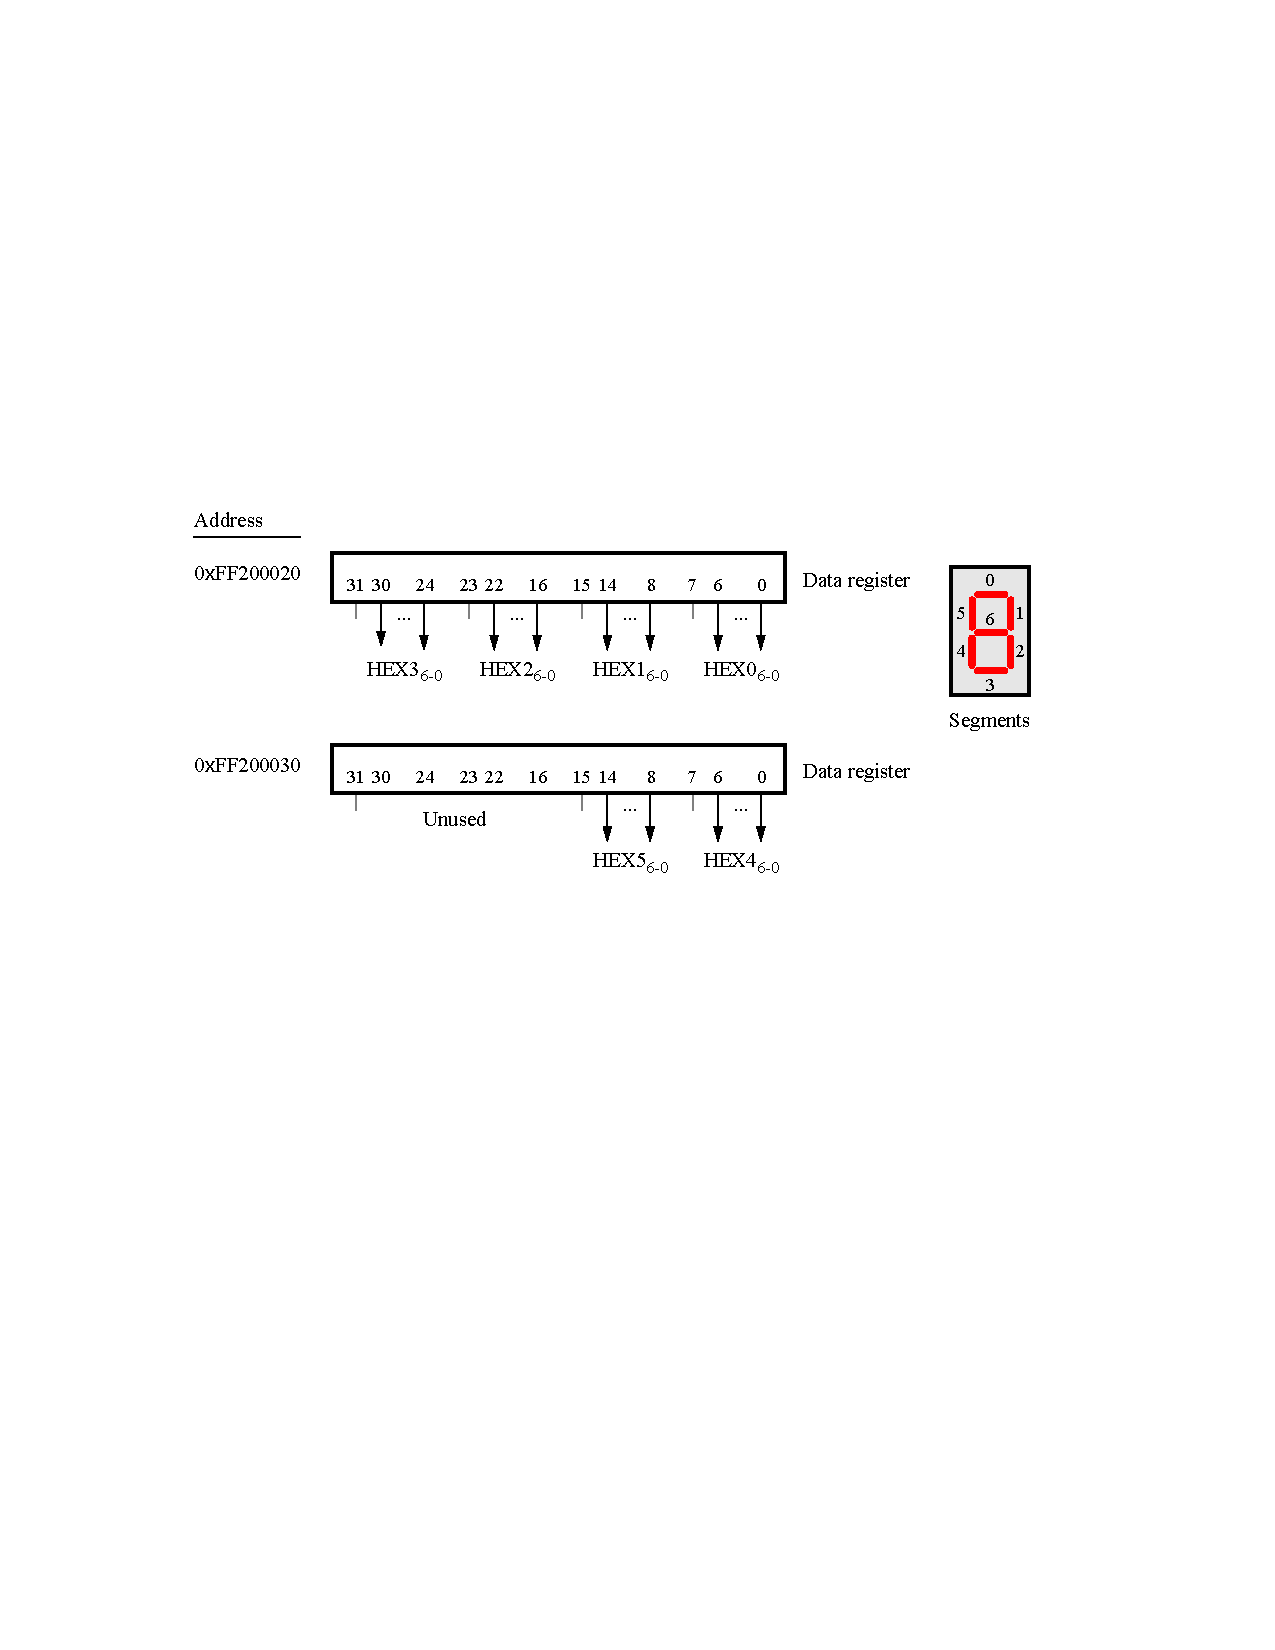
\includegraphics{figures/fig_segment_port.pdf}
   \end{center}
	\caption{The seven-segment display ports.}
\label{fig:segment}
\end{figure}


\noindent
As an alternative to seven-segment displays, you can use the Linux* Terminal window. In
this case, you should designate a six-character space on the display in which to show the
message. You can ``draw'' a box using ASCII characters as illustrated below:

\begin{lstlisting}
         ------
        |      |
         ------
\end{lstlisting}

\noindent
If the message is scrolled inside of this box, the effect will be similar in appearance to
using (six) seven-segment displays. Some Terminal window commands are listed in
Table~\ref{tab:vt100}. For 
example, the command \texttt{$\backslash$e[2J} clears the Terminal window, and the 
command \texttt{$\backslash$e[H} moves the Terminal {\it cursor} to the {\it home} position in 
the upper-left corner of the window.  In these commands \texttt{$\backslash$e} represents 
the \texttt{Escape} character. It can alternatively be specified by its ASCII code, using 
the syntax \texttt{$\backslash$033}. You can send such commands to the Terminal window by 
using the \texttt{printf} function. For example, the Terminal window can be cleared by calling 

\begin{lstlisting}
printf ("\e[2J");			// clear Terminal window
fflush (stdout);
\end{lstlisting}

\noindent
Additional Terminal window commands can be found by searching on the Internet for
\texttt{VT100 escape codes}.
\begin{table}[h]
\caption{Terminal window ASCII commands.}
~\\
\centering
\label{tab:vt100}
\begin{tabular}{l|l}
		  {\bf Command} & {\bf Result} \\ \hline
		  \rule{0cm}{.375cm}\texttt{$\backslash$e7} & save cursor position and attributes\\
		  \texttt{$\backslash$e8} & restore cursor position and attributes\\
		  \texttt{$\backslash$e[H} & move the cursor to the home position\\
		  \texttt{$\backslash$e[?25l} & hide the cursor \\
		  \texttt{$\backslash$e[?25h} & show the cursor \\
		  \texttt{$\backslash$e[2J} & clear window \\
		  \texttt{$\backslash$e[ccm} & set foreground color to \texttt{cc}$^1$ \\
		  \texttt{$\backslash$e[yy;xxH} & set cursor location to row \texttt{yy}, column \texttt{xx}
		  
\end{tabular}
\end{table}

\noindent
For both seven-segment displays and the Terminal window, use a delay when scrolling the message 
so that the letters shift to the left at a reasonable speed. To implement the required delay you 
can use a Linux library function such as \texttt{nanosleep}. 

~\\
\noindent
Perform the following:

\begin{enumerate}
\item Create a file called {\it part1.c} and type your C code into this file. Whether you are 
using seven-segment displays or the Terminal window, your code should be mostly the same. In 
one case, you write six characters at a time from the message to the seven-segment display 
ports, and in the other case you print these same characters (inside the box) on the 
Terminal window. 

You should provide the ability to pause or run the scrolling operation by using the pushbutton 
KEYs. The programming registers in a DE-series KEY port are illustrated in Figure~\ref{fig:KEY}.
There is a {\it Data} register that reflects which KEY(s) are pressed at a given time. For 
example, if {\it KEY}$_0$ is currently being pressed, then bit 0 of the data register will be~1,
otherwise~0. The {\it Edgecapture} register can be used to check if a {\it KEY} has been 
pressed since last examined, even if it has since been released. If, for example, 
{\it KEY}$_0$ is pressed then bit 0 of the {\it Edgecapture} register becomes~1 and 
remains so even if {\it KEY}$_0$ is released. To reset the bit to 0, a program has to 
explicitly write the value~1 into this bit-position of the {\it Edgecapture} register. 
The {\it Interruptmask} register is not used for this exercise, and can be ignored.

\begin{figure}[H]
   \begin{center}
       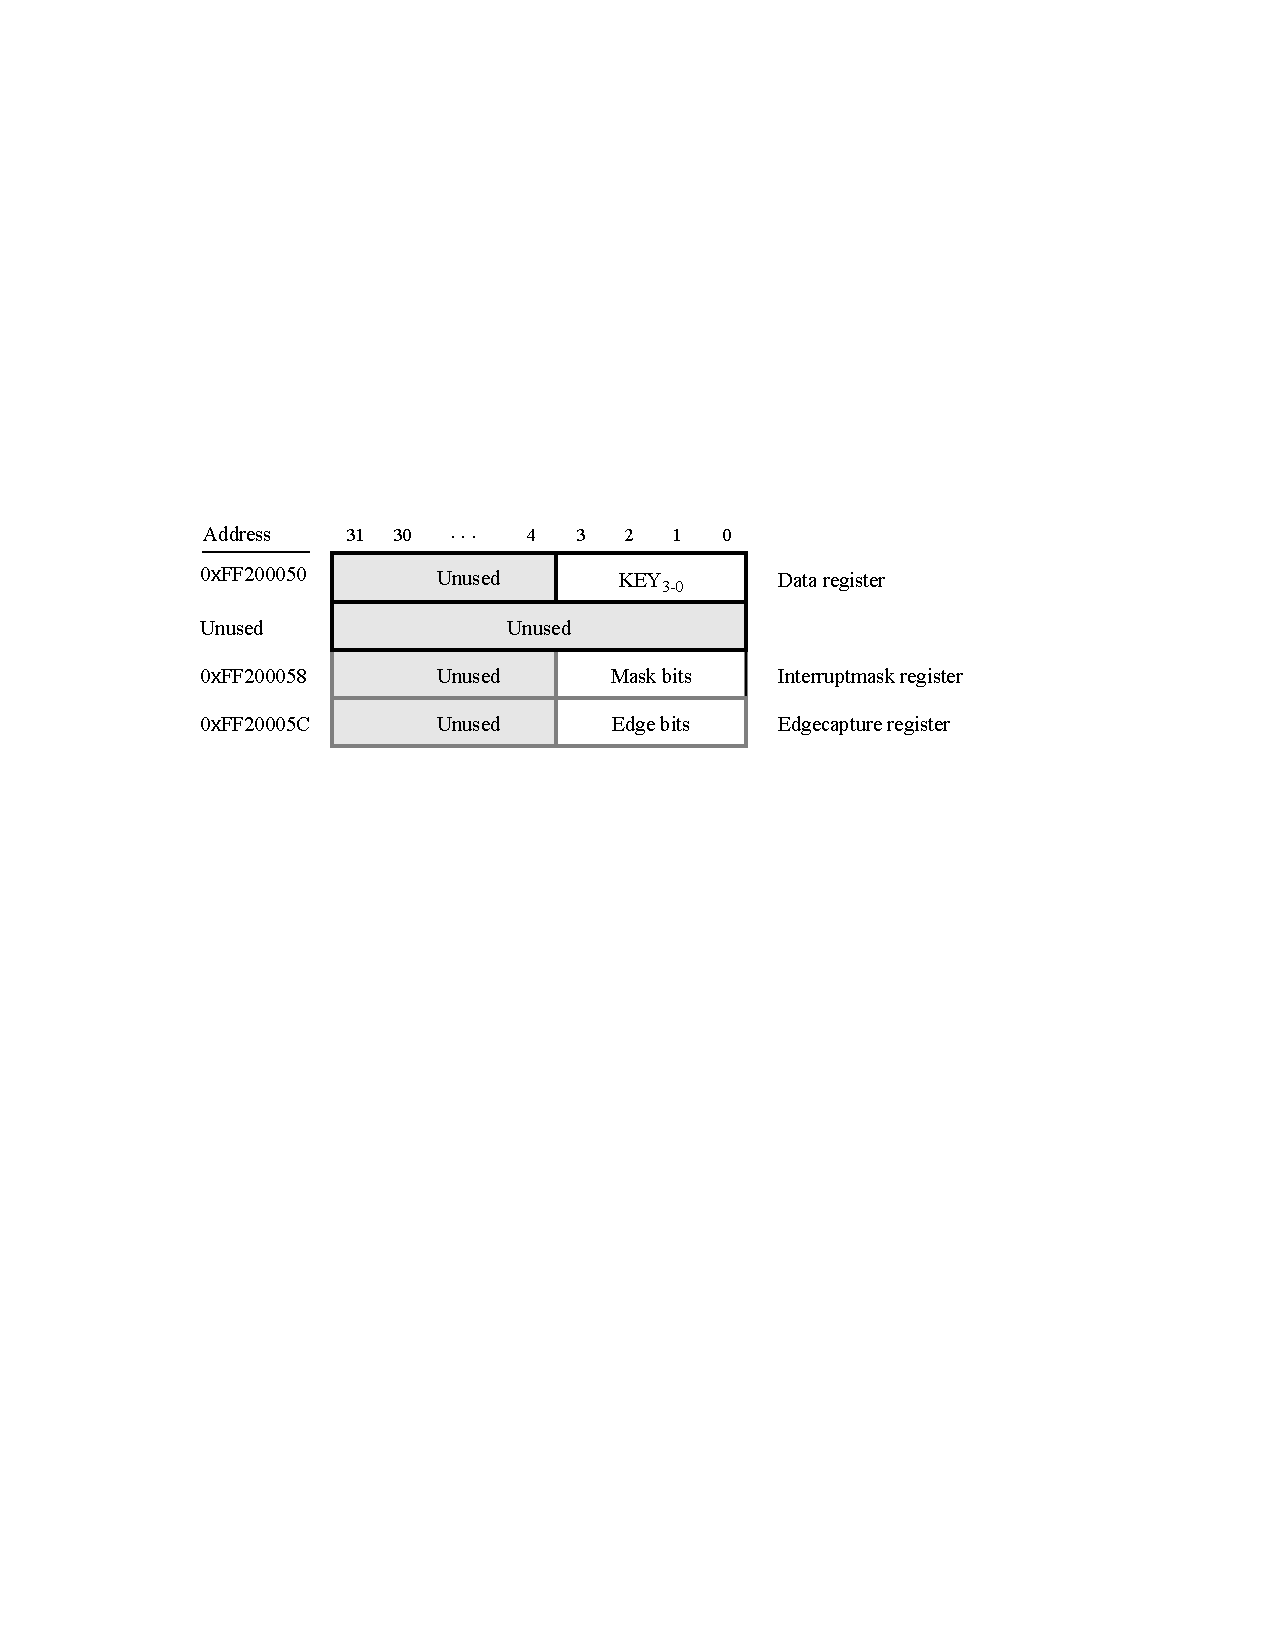
\includegraphics{figures/fig_KEY_port.pdf}
   \end{center}
   \caption{The pushbutton KEY port.}
	\label{fig:KEY}
\end{figure}

To communicate with the KEYs, and seven-segment displays if applicable, use memory-mapped 
I/O as explained in the tutorial {\it Using Linux on DE-series Boards}. The source code from 
this tutorial for translating physical addresses into virtual addresses is included along with 
this laboratory exercise. You can use this source code as part of your solution.

\item
Compile your code using a command such as \texttt{gcc -Wall -o part1 part1.c}.
\item
Execute and test your program.
\end{enumerate}

\section*{Part II}
\noindent
In Lab Exercise 1 you were asked to write a kernel module to control the LED lights and
to display a digit, either on a seven-segment display or the Terminal window. 
The kernel module responded to interrupts
generated by the KEY pushbutton port. Here you are to write another interrupt-driven
kernel module.

~\\
\noindent
Your kernel module should implement a real-time clock. Display the time on seven-segment
displays, if available, or in the Terminal window. The time
should be displayed in the format \red{MM}:\red{SS}:\red{DD}, where \red{{\it MM}} are minutes, 
\red{{\it SS}} are seconds, and \red{{\it DD}} are hundredths of a second. 
To keep track of time you
should use a {\it hardware timer} module. The DE-series computers include a 
number of hardware timers.  For this exercise use an interval timer implemented 
in the FPGA called {\it FPGA Timer0}.
The register interface for this timer has the base address {\sf 0xFF202000}. As shown in 
Figure~\ref{fig:timer} this timer has six 16-bit registers. To use the timer you need
to write a suitable value into the {\it Counter start value} registers (there are two, one for the
upper 16~bits, and one for the lower 16 bits of the 32-bit counter value). To start the
counter, you need to set the {\it START} bit in the {\it Control} register to~1. Once
started the timer will count down to~0 from the initial value in the {\it Counter start
value} register.  The counter will automatically reload this value and continue counting 
if the {\it CONT} bit in the {\it Control} register is~1. When the counter reaches~0,
it will set the {\it TO} bit in the {\it Status} register to~1. This bit can be cleared 
under program control by writing a~0 into it. If the {\it ITO} bit in the control register is 
set to~1, then the timer will generate an ARM* processor interrupt each time 
it sets the {\it TO} bit.
The timer clock frequency is 100~MHz. The interrupt~ID of the timer is~72.
Follow the instructions in the tutorial {\it Using Linux on DE-series Boards} to register this
interrupt~ID with the Linux kernel and ensure that it invokes your kernel module whenever
the interrupt occurs.

~\\
\begin{figure}[htb]
	\begin{center}
	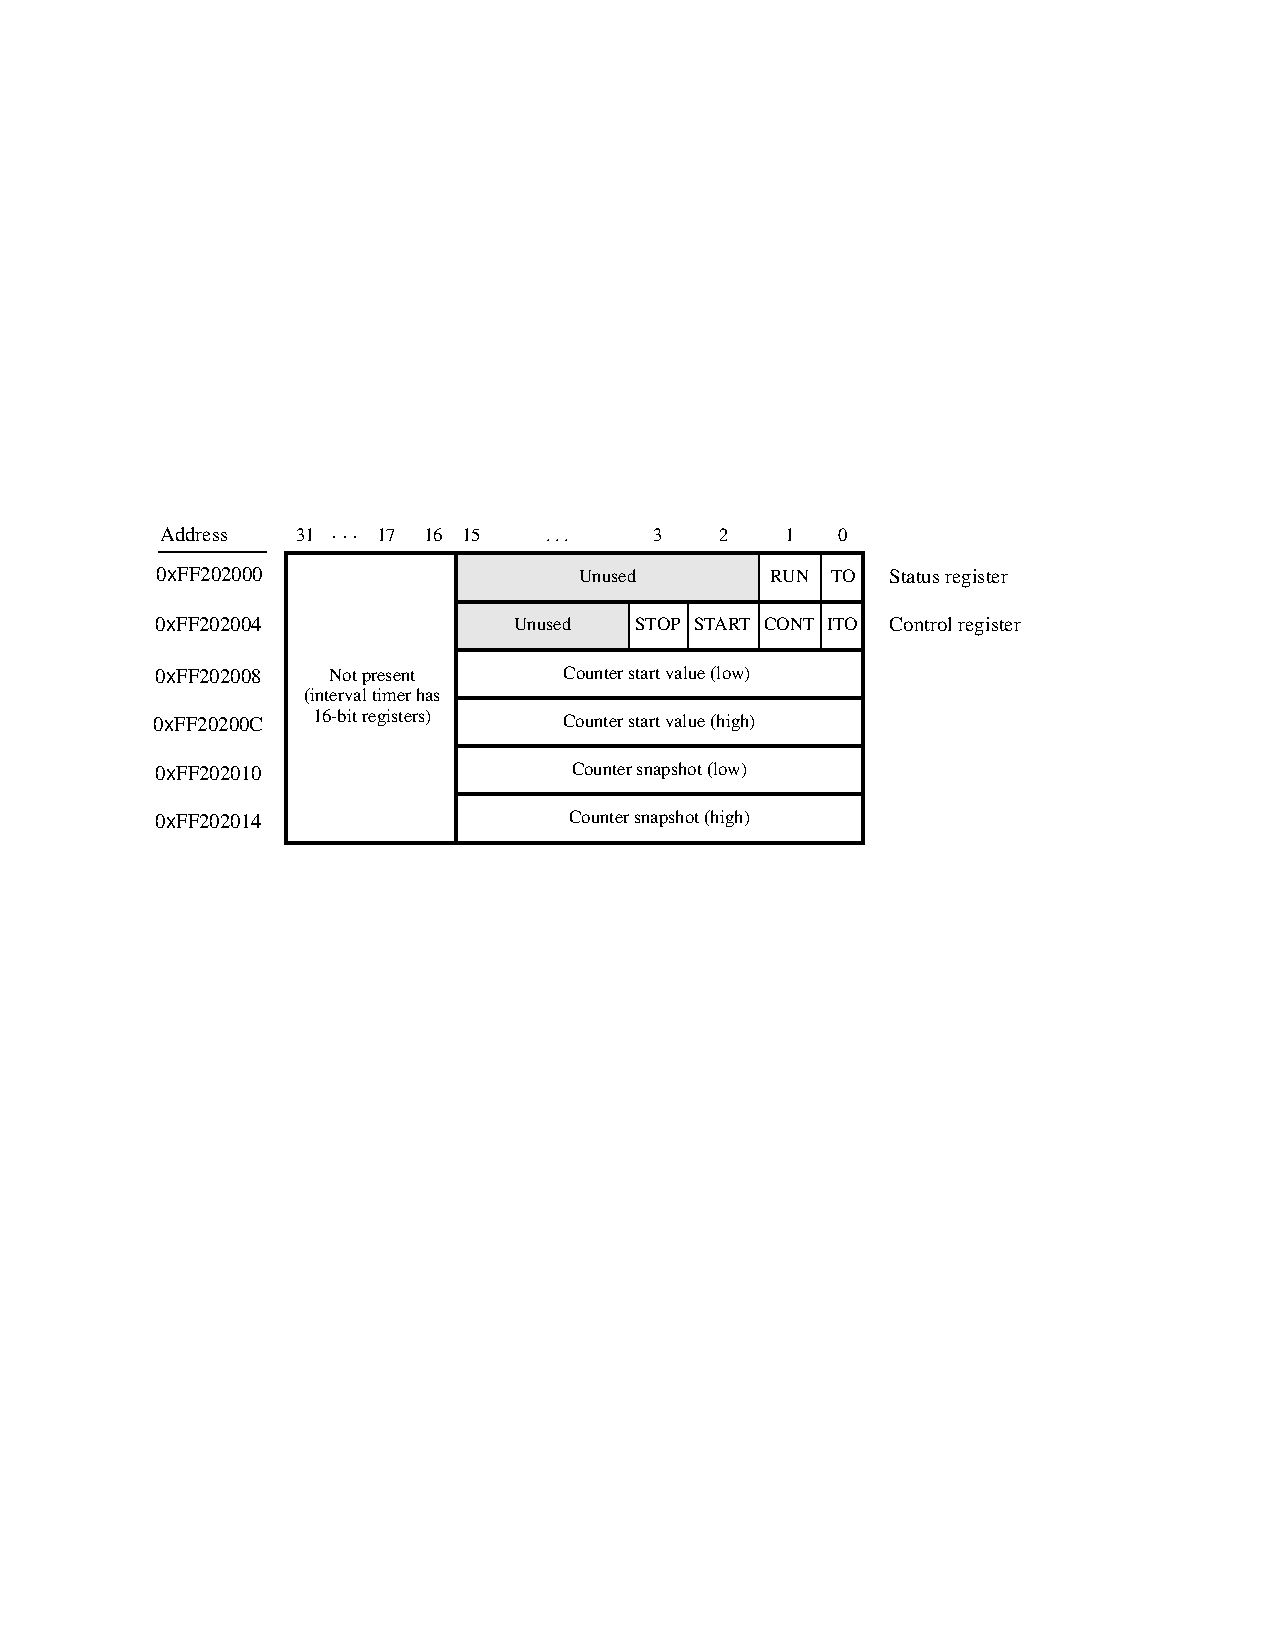
\includegraphics[scale=1]{figures/fig_interval_port.pdf}
	\end{center}
	\caption{The {\it FPGA Timer0} register interface.}
\label{fig:timer}
\end{figure}

\noindent
Perform the following:

\begin{enumerate}
\item Create a file called {\it timer.c} and type your C code into this file.

\item
Create a suitable {\it Makefile} that can be used to compile your kernel module and create the 
file {\it timer.ko}. Insert this module into the kernel using the command \texttt{insmod timer.ko}.
Each time an interrupt occurs your interrupt-service routine should increment the value of the 
time. When the time reaches \red{59}:\red{59}:\red{99}, it should wrap around to 
\red{00}:\red{00}:\red{00}. 

If using seven-segment displays, you can continuously display the updated time. But if
using the Terminal window, it is better to print the time only when the user requests it.
For example, your timer interrupt service routine could read from the KEY port and print the 
time whenever {\it KEY}$_1$ has been pressed.

You can remove your module from the Linux kernel by using the command 
\texttt{rmmod timer}. When removed, your {\it exit} routine should clear the seven-segment
diplays, if applicable.
\end{enumerate}

\section*{Part III}
\noindent
For this part you are to write a kernel module that implements a {\it stopwatch}. The stopwatch
time should be shown either on seven-segment displays or the Terminal window. The time should 
be settable using the SW switches and KEY pushbuttons in your DE-series Computer. The time 
should be displayed in the format \red{MM}:\red{SS}:\red{DD} as was done for Part II.
Implement the stopwatch module using two sources of interrupts: the hardware timer 
{\it FPGA Timer0} and the KEY pushbutton port. For each timer interrupt you should 
{\it decrement} the stopwatch until it reaches \red{00}:\red{00}:\red{00}.

~\\
\noindent
The behavior of the interrupt service routine for the pushbutton KEY port depends on which
DE-series board is being used. If you are using the DE1-SoC or DE10-Standard board, then
follow the instructions in Table~\ref{tab:action1}. For the DE10-Nano board, which has
fewer KEYs and SW switches, implement the actions given in Table~\ref{tab:action2}.

\begin{table}[h]
\caption{Interrupt actions for the DE1-SoC and DE10-Standard boards.}
~\\
\centering
\label{tab:action1}
\begin{tabular}{c|p{13cm}}
{\bf KEY} & {\bf Action} \\ \hline
\rule{0cm}{.375cm}{\it KEY}$_0$ & Toggle the stopwatch to be either running or paused \\
{\it KEY}$_1$ & When pressed, use the values of the SW switches to set the \red{DD} part of the 
stopwatch time. The maximum value is \red{99} \\
{\it KEY}$_2$ & When pressed, use the values of the SW switches to set the \red{SS} part of the 
stopwatch time. The maximum value is \red{59} \\
{\it KEY}$_3$ & When pressed, use the values of the SW switches to set the \red{MM} part of the 
stopwatch time. The maximum value is \red{59} \\
\end{tabular}
\end{table}


\begin{table}[h]
\caption{Interrupt actions for the DE10-Nano board.}
~\\
\centering
\label{tab:action2}
\begin{tabular}{c|p{13cm}}
{\bf KEY} & {\bf Action} \\ \hline
\rule{0cm}{.375cm}{\it KEY}$_0$ & Toggle the stopwatch to be either running or paused \\
{\it KEY}$_1$ & If the stopwatch is running, just print the current time on the Terminal
window. But if the stopwatch is stopped, then set the time using the SW switch values. Set 
one stopwatch digit
each time {\it KEY}$_1$ is pressed, in a specific sequence. 
For the first press, set the right digit of \red{DD},
for the second press set the left digit of \red{DD}, for the third press set the right
digit of \red{SS}, and so on. After each press of {\it KEY}$_1$ print the current stopwatch time.
\end{tabular}
\end{table}

~\\
\noindent
The data register in the SW switch port for the DE1-SoC and DE10-Standard boards is shown in 
Figure~\ref{fig:slider}. The SW switch port for the DE10-Nano board, not shown in the figure, 
has only four switches {\it SW}$_0$ to {\it SW}$_3$. 

\begin{figure}[H]
   \begin{center}
       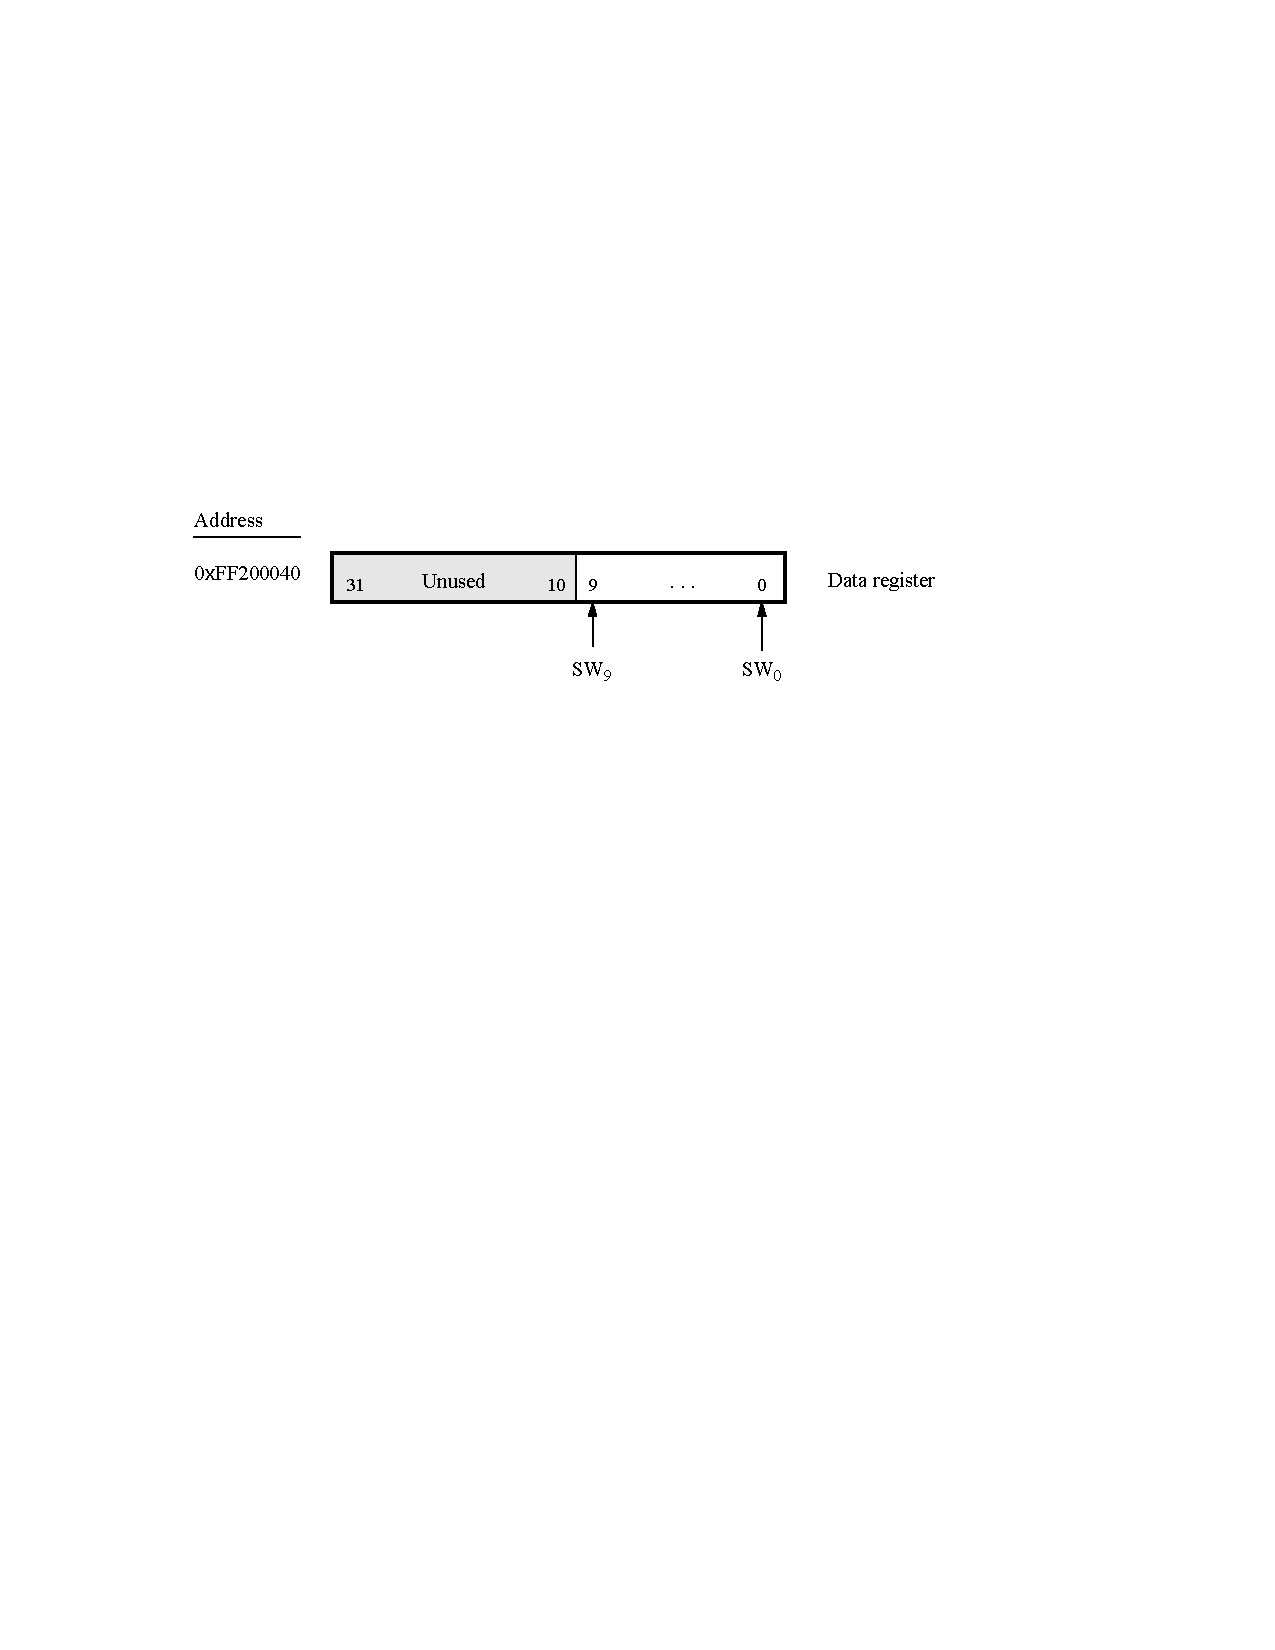
\includegraphics{figures/fig_slider_port.pdf}
   \end{center}
	\caption{The SW switch port.}
\label{fig:slider}
\end{figure}

\noindent
Perform the following:

\begin{enumerate}
\item Create a file called {\it stopwatch.c} and type your C code into this file.

\item
Create a suitable {\it Makefile} that can be used to compile your kernel module and create the 
file {\it stopwatch.ko}. Ensure that the {\it timer} module from Part II has already been 
removed from the kernel, because it also responds to interrupts from FPGA Timer0. Then, 
insert the stopwatch module into the kernel by using the 
command \texttt{insmod stopwatch.ko}. 

If you are using seven-segment displays, then as soon as the module is inserted you should 
see the time \red{59}:\red{59}:\red{99} start to decrement on the displays. But if you are
using the Terminal window, then you should see the stopwatch time whenever the user presses
{\it KEY}$_1$.
\end{enumerate}

~\\
\noindent
You can remove your module from the Linux kernel by using the command 
\texttt{rmmod stopwatch}. When removed, your {\it exit} routine should clear the seven-segment
displays, if applicable.
\vskip 0.8in
\noindent
\newpage
%%%%%%%%%%%%%%%%%%%%%%%%%%%%%%%%%%%%%%%%
%%% FPGAcademy Copyright Information %%%
%%%%%%%%%%%%%%%%%%%%%%%%%%%%%%%%%%%%%%%%

%Always put the copyright on a new page (clear page), with some vertical space from top
\clearpage
\vspace{1in}

\noindent

Copyright {\copyright} FPGAcademy.org. All rights reserved. FPGAcademy and the 
FPGAcademy logo are trademarks of FPGAcademy.org.  This document is provided 
"as is", without warranty of any kind, express or implied, including but not 
limited to the warranties of merchantability, fitness for a particular purpose 
and noninfringement. In no event shall the authors or copyright holders be 
liable for any claim, damages or other liability, whether in an action of 
contract, tort or otherwise, arising from, out of or in connection with the 
document or the use or other dealings in the document.
~\\
~\\
**Other names and brands may be claimed as the property of others.



\end{document}
